\documentclass[12pt,letterpaper]{article}
\usepackage{fullpage}
\usepackage[top=2cm, bottom=4.5cm, left=2.5cm, right=2.5cm]{geometry}
\usepackage{amsmath,amsthm,amsfonts,amssymb,amscd}
\usepackage{lastpage}
\usepackage{enumerate}
\usepackage{fancyhdr}
\usepackage{mathrsfs}
\usepackage{xcolor}
\usepackage{graphicx}
\usepackage{listings}
\usepackage{hyperref}

\lstset{columns=fullflexible}

\hypersetup{%
  colorlinks=true,
  linkcolor=blue,
  linkbordercolor={0 0 1}
}
 
\renewcommand\lstlistingname{Algorithm}
\renewcommand\lstlistlistingname{Algorithms}
\def\lstlistingautorefname{Alg.}

\lstdefinestyle{Python}{
    language        = Python,
    frame           = lines, 
    basicstyle      = \footnotesize\ttfamily,
    keywordstyle    = \color{blue},
    stringstyle     = \color{green},
    commentstyle    = \color{red}\ttfamily
}

\lstdefinestyle{Bash}{
   basicstyle=\footnotesize\ttfamily,
   stringstyle=\color{red},
   keywordstyle=\color{blue},
   commentstyle=\color{darkgrey}\slshape,
   morekeywords={linestyle,linetype,linewidth,linecolor,pointtype,nohidden3d,hidden3d,palette,lt,lw,lc,pt,ps,fd,fill,fs,ls},
   framexleftmargin=1mm, framextopmargin=1mm, frame=single
 }
 
 \lstdefinestyle{BBash}{
   backgroundcolor=\color{lightgray},
   basicstyle=\footnotesize,
   stringstyle=\color{red},
   keywordstyle=\color{blue},
   commentstyle=\color{darkgrey}\slshape,
   morekeywords={linestyle,linetype,linewidth,linecolor,pointtype,nohidden3d,hidden3d,palette,lt,lw,lc,pt,ps,fd,fill,fs,ls},
   framexleftmargin=1mm, framextopmargin=1mm, frame=single
 }

\lstdefinestyle{C++}{
    language        = C++,
    frame           = lines, 
    basicstyle      = \footnotesize,
    keywordstyle    = \color{blue},
    stringstyle     = \color{green},
    commentstyle    = \color{red}\ttfamily
}

\setlength{\parindent}{0.0in}
\setlength{\parskip}{0.05in}


\pagestyle{fancyplain}
\headheight 35pt

\chead{\textbf{\Large ExaHyPE 2 Tutorial}}
\rhead{ \today}
\lfoot{}
\cfoot{}
\rfoot{\small\thepage}
\headsep 1.5em

\begin{document}

\begin{figure}[!h]
\centering

\includegraphics[width=0.5\linewidth]{pictures/ExaHyPE_Logo.jpg}
\end{figure}

\section{Introduction}
\label{sec:Introduction}

\vspace{0.2cm}

This document is meant to be an introductory tutorial into ExaHyPE 2. ExaHyPE 2 is part of \textbf{Peano4}, which is an open source framework for solvers on dynamically adaptive Cartesian meshes that was developed by a team led by Tobias Weinzierl, who is at the time of writing Professor at the department of Computer Science of Durham University in the United Kingdom.\\ \\
\textbf{ExaHyPE} itself is a hyperbolic PDE engine, its goal is to provide a generic engine in which users can implement the specifics of their hyperbolic PDEs and have these be solved by the engine. This is what we will endeavor to do in the following. \\
ExaHyPE solves partial differential equations of the following form: \\ 

\begin{equation*}
    \frac{\partial Q}{\partial t} + \nabla . F(Q, \nabla Q) + B(Q) . \nabla Q= S(Q) + \sum_{i = 1}^{n_{ps}} \delta_i
\end{equation*}

Here $F$ is called the \textit{flux} $B$ is the \textit{non-conservative product} (often shortened to \textit{NCP}) and $S$ is the \textit{source} of the equation.\\
For simplicity the easiest way to think of each of these is as follows:
\begin{itemize}
	\item The flux contains terms linked to the transmission of a quantity within the domain such as the flow of heat from a hot part of the domain to a colder one. It concerns quantities that do not change but merely move from part to another.
	\item The NCP, as the term \textit{non-conservative} would imply, contains terms that are transmitted but can increase or decrease. One example for this would be friction, which causes the overall velocity of the system to decrease.
	\item The Source contains terms that are acted upon the system from outside, such as gravity or someone acting upon it.
\end{itemize}

\textbf{Acknowledgments}:
ExaHyPE 2 is the follow-up development of the ExaHyPE project which has been funded
by the EU from 2015–2019.\\
Thank you to Tobias Weinzierl, who has been a cornerstone of this project since its inception. Thank you as well to Derek Aguiar, whose template was used in making this document. \\

\textbf{Additional documentation} about the project, including information about some of the algorithms or design choices, can be found in the guidebook which comes included with Peano4. This can be compiled from source using the files in the folder \textbf{documentation} that is located in Peano4's root directory.

\newpage


\section{Verifying the installation and building a project}
\label{Verifying_and_building}

The first requirement to using any of the ExaHyPE2 applications is a succesful compilation of the Peano libraries that it is based on. There are two ways to compile these: the first is using autotools and the configure script, the second is using cmake. Only the first will be expanded upon here but both should lead the same results.\\

First, navigate to the Peano root directory, this is typically simply called \textbf{Peano}. Then ensure that all \textbf{autotools} packages are installed on your system, these are typically shipped in the packages \textbf{autoconf, automake \& libtool} and can be installed as follows:\\

\begin{lstlisting}[style = Bash]
sudo apt-get install autoconf automake libtool
\end{lstlisting}

then, use these to set up the configure environment as follows:

\begin{lstlisting}[style = Bash]
libtoolize; aclocal; autoconf; autoheader;
cp src/config.h.in .;
automake --add-missing
\end{lstlisting}

this should generate a number of files which will enable us to configure which optional parts of Peano we want to use using the configure command. For ExaHyPE we require at least the ExaHyPE as well as blockstructured and loadbalancing toolboxes. In order to improve the compilation speed we can additionally enable multithreading. A basic configuration would look as follows:

\begin{lstlisting}[style = Bash]
./configure --enable-exahype --enable-blockstructured --enable-loadbalancing \
    --with-multithreading=omp
\end{lstlisting}

Finally we can compile Peano, to do this simply invoke the \textit{make} command:

\begin{lstlisting}[style = Bash]
make -j8
\end{lstlisting}

This may take a few minutes. Once it is done, we have one final thing we have to do before we can run our first ExaHyPE application: configure our python environment. ExaHyPE uses python code as an API in order to generate the applications according to the users' instructions. This requires a few python packages, but we also need to let our machine know where to look for the python code, to do this, simply run:

\begin{lstlisting}[style = Bash]
pip3 install jinja2 sympy
export PYTHONPATH=../../../python
\end{lstlisting}

Finally we can build our first project:

\begin{lstlisting}[style = Bash]
python3 example_scripts/Advection.py
\end{lstlisting}

Assuming this was succesfull, you should see a number of files have appeared in your working directory. We will ignore most of these for now, but know that these contain the implementation of the ExaHyPE 2 simulation.\\
One file in particular is of interest to us now: the file simply named Advection2D is the executable for our implementation. We will therefore run this executable file by using the following command:

\begin{lstlisting}[style = Bash]
./Advection2D
\end{lstlisting}

which should hopefully run succesfully. You can make sure of this by checking that a number of files with the prefix: "\textbf{solution-advection}" have appeared in the directory \textit{solutions}. These contain the solution of our problem, which we will take a look at as soon as we have an understanding of how our problem is defined.

\newpage

\section{Our first Configuration file}
\label{section_3}


We should now have executed our first ExaHyPE 2 application, but in order to understand what it is that we have executed, let us take a look at the file which defined this application: \textbf{Advection.py}, which can be found in the folder \textit{example\_scripts}\\
As mentioned in the \hyperref[sec:Introduction]{Introduction}, the configuration files are in python, so it should surprise noone that they start with the following:

\begin{lstlisting}[style = Python]
import peano4
import exahype2
\end{lstlisting}

These merely import the necessary packages from Peano4 and ExaHyPE 2 which will let us define and build our project. Speaking of defining our project, this happens in the next step:\\

\begin{lstlisting}[style = Python]
project = exahype2.Project(
    ["examples", "exahype2", "tutorial"],
    "advection",
    ".",
    executable="Advection" + str(dimensions) + "D"
)
\end{lstlisting}

The parameters here are as follows: first the namespace that the project will have in C++, then the name of the project itself, then where the project should be generated and finally the name of the executable.
Next we will define and add a solver to this project:\\

\begin{lstlisting}[style = Python]
thesolver = exahype2.solvers.fv.rusanov.GlobalAdaptiveTimeStep(
    "advection",
    patch_size=3,
    unknowns=3, auxiliary_variables=0,
    min_volume_h=0.01, max_volume_h=0.03,
    flux = exahype2.solvers.fv.PDETerms.User_Defined_Implementation,
    time_step_relaxation = 0.1
)
\end{lstlisting}

most of this should be self-explanatory and some pieces will be explained in more detail later, but a few things deserve special mention here.\\
First is the solver itself, the type \textit{ExaHyPE2.solvers.fv.rusanov.GlobalAdaptiveTimeStep()} indicates the type of solver. \textbf{fv} stands for \textbf{finite volumes}, this describes the type of the solver, rusanov is the type of flux that is used to solve the riemann problem at boundaries between cells. Finally global adaptive time step means the solver automatically chooses an appropriate time step and uses this same time step over the entire domain.\\
For the parameters of this solver: "\textit{name="advection"}", this determines the name of the project and therefore of the files generated by ExaHyPE 2 that will define the application. "\textit{unknowns=3}" and "\textit{auxiliary\_variables=0}" define the variables of our equation, in this case we have a partial differential equation with 3 component variables but no auxiliary variables, which are parameters that can be space-dependent but don't change for the duration of the simulation.\\ 
The last thing worth mentioning is the parameter \textit{flux} which we have here set to some user defined implementation. We will need to define this in a subsequent step.
\newpage

Next we define the parameters for our simulation, this is where we define the volume of our domain and the number of dimensions for example, but also where basic information about the plotting behaviour is defined:
\begin{lstlisting}[style = Python]
project.set_global_simulation_parameters(
    dimensions = 2,
    offset = [0.0,0.0],
    size = [1.0,1.0],
    min_end_time = 0.5,
    max_end_time = 0.5,
    first_plot_time_stamp = 0.0,
    time_in_between_plots = 0.025, # snapshots
    periodic_BC = [False, False, False]
)
\end{lstlisting}

Finally, given all the information above we can generate and build a working application.

\begin{lstlisting}[style = Python]
build_mode = peano4.output.CompileMode.Release
project.set_load_balancing(
    "toolbox::loadbalancing::RecursiveSubdivision",
    "new ::exahype2::LoadBalancingConfiguration()"
)
project.set_Peano4_installation( "../../../", build_mode )
peano4_project = project.generate_Peano4_project(False)
peano4_project.build(make_clean_first=True, number_of_parallel_builds=4)
)\end{lstlisting}

Logically, this application is still missing some information about the implementation of this PDE. We mentioned that we would need to define the flux, but we have also not yet defined any initial conditions or boundary conditions.\\
We will do so in the next step.

\newpage

\section{Our first implementation file}

The astute reader might have noticed that before we built our project, there were already a few files in the containing folder, most noticeably one that has to do with the project they just built: \textbf{advection.cpp}. We will be taking a look at this file next since, as you most likely have already guessed, it contains the implementation of our PDE.
\\ \\
Before we do this however, we will quickly define the PDE that is to come. As the name of the file will have already indicated, this is the advection equation. This is one of the simplest equations we can possibly define and it appears as follows:

\begin{equation*} \label{Advection_equation}
    \frac{\partial}{\partial t}\left(
    \begin{array}{lr} q_x \\
                      q_y \\
                      q_z 
                      \end{array} \right) +
    \nabla \begin{pmatrix}
                      q_x  & 0   & 0 \\
                      0    & q_y & 0 \\
                      0    & 0   & q_z 
    \end{pmatrix}  = \vec{0}
\end{equation*}

This equation describes the transport of a quantity $q$ by the motion of a fluid, such as the movement of a particle in a river. \\
In order to implement this equation, four things are needed: the initial condition, the boundary conditions, the maximal eigenvalue and the flux.\\

We start with the initial conditions: here we define a starting configuration in which the quantity in direction $i$ is equal to the position in that direction $x_i$.\\

\begin{lstlisting}[style = C++]
void examples::exahype2::tutorial::advection::initialCondition(
  double * __restrict__ Q,
  const tarch::la::Vector<Dimensions,double>&  volumeCentre,
  const tarch::la::Vector<Dimensions,double>&  volumeH,
  bool                                         gridIsConstructred
) {

  for (int i=0; i<NumberOfUnknowns+NumberOfAuxiliaryVariables; i++) {
    Q[i] = volumeCentre[i];
  }

}
\end{lstlisting}

\newpage


Next we can define the largest eigenvalue of our system. This is important because it defines a lot of the behaviour of the PDE, and among others the maximum allowable timestep for which a lot of solvers remain stable. The eigenvalues of the advection equations are equal to the velocity of the fluid, which here we set uniformly to 1:

\vspace{1cm}

\begin{lstlisting}[style = C++]
double ::examples::exahype2::tutorial::advection::maxEigenvalue(
  const double * __restrict__ Q, // Q[3+0],
  const tarch::la::Vector<Dimensions,double>&  faceCentre,
  const tarch::la::Vector<Dimensions,double>&  volumeH,
  double                                       t,
  double                                       dt,
  int                                          normal
)  {

  return 1.0;

}
\end{lstlisting}

\vspace{1cm}


Next, let's define our flux in x and y direction according to our \hyperref[Advection_equation]{previous definition}.
The directions of the flux are defined by the normal parameter. This parameter defines through which surface, and therefore in which direction, the flux is being computed. Here if the normal is \textbf{0}, we are computing the flux in x direction and if the normal is \textbf{1}, we are computing the flux in y direction. For higher dimensions, there would logically be additional directions to implement the flux in.

Our fluxes in x and y directions are:

\begin{equation*}
    F_x = \begin{pmatrix}
                      u_x \\
                      0 \\
                      0
    \end{pmatrix}, \hspace{\fill} 
    F_y =\begin{pmatrix}
                      0 \\
                      u_y \\
                      0
    \end{pmatrix}
\end{equation*}\\

Which we implement as:

\newpage

\begin{lstlisting}[style = C++]
void ::examples::exahype2::tutorial::advection::flux(
  const double * __restrict__ Q, // Q[3+0],
  const tarch::la::Vector<Dimensions,double>&  faceCentre,
  const tarch::la::Vector<Dimensions,double>&  volumeH,
  double                                       t,
  double                                       dt,
  int                                          normal,
  double * __restrict__ F // F[3]
)  {
	
  if(normal==0){
    F[0] = Q[0];
    F[1] = 0.0;
    F[2] = 0.0;
  else if(normal==1){
    F[0] = 0.0;
    F[1] = Q[1];
    F[2] = 0.0;
  }
  
}
\end{lstlisting}


Finally, we can define our boundary conditions. For this simple case, we will simply use reflecting boundary conditions. This means all values except the density will be the same outside of the as inside of it.\\ \\


\begin{lstlisting}[style = C++]
void examples::exahype2::tutorial::advection::boundaryConditions(
  const double * __restrict__                  Qinside, // Qinside[3+0]
  double * __restrict__                        Qoutside, // Qoutside[3+0]
  const tarch::la::Vector<Dimensions,double>&  faceCentre,
  const tarch::la::Vector<Dimensions,double>&  volumeH,
  double                                       t,
  int                                          normal
) {

  for(int i=0; i<3; i++){
    Qoutside[i] = Qinside[i];
  }

}
\end{lstlisting}

And that is all there is to it, all that was needed was one file defining our problem and four small functions defining how to compute it. \\
But now that we have computed our problem, we'd like to visualize it.\\
We will do so in the next (very short) section.

\newpage

\section{Visualizing results from ExaHyPE}
\label{Visualize}

\vspace{0.3cm}

Peano 4 and therefore ExaHyPE per default write the results in a native format. These are defined by two files, a more general one called \textbf{solution-\textit{project\_name}.peano-patch-file} and individual ones for each logged time step called \textbf{solution-\textit{p}-\textit{file\_number}-rank-\textit{rank\_number}.peano-patch-file}.\\
The first of these two just contains information linking each file of the second type to a specific timestamp, it allows an interpreter to find the other files and assign them to the proper location and time. The second type contains the values computed in each patch as an array which contains one after another the values of each variable for each cell in the patch. The patches are specified by their position and size.\\
This relatively simple, machine readable format allows one to easily create applications for processing and visualising these results oneself. A few of these are provided with Peano 4 as is.

In our case, we will just mention how to convert these to VTU format, which would allow one to read them with paraview for example, the most commonly used application for scientific visualization.
To do so, simply use the command:
\begin{lstlisting}[style = Bash]
pvpython path_to_peano4/python/peano4/visualization/render.py \
solutions/solution-project_name.peano-patch-file
\end{lstlisting}
with the corresponding path to the Peano 4 installation directory and project name. In the case of our previous example, this would be:
\begin{lstlisting}[style = Bash]
pvpython ../../../python/peano4/visualization/render.py \
 solutions/solution-advection.peano-patch-file
\end{lstlisting}
For our aforementioned example, we can see how the quantites are shifted along the domain:

\begin{figure}[!h]
\centering
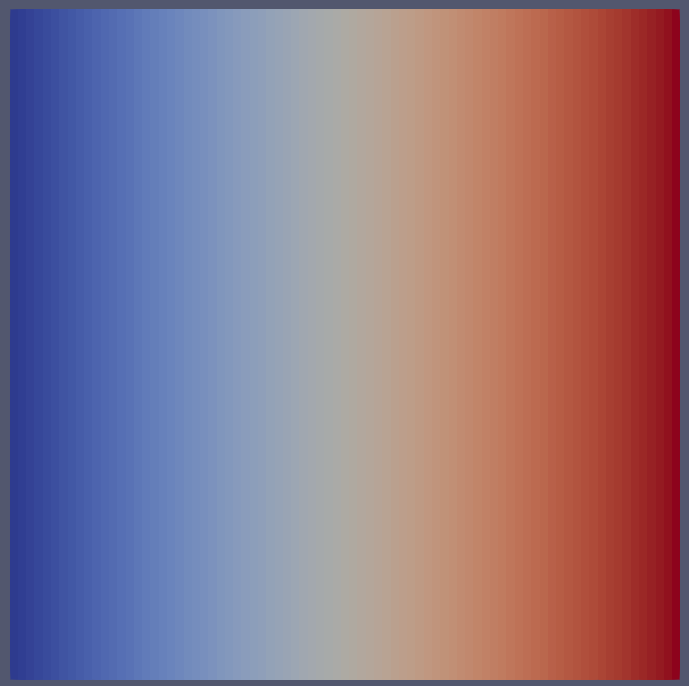
\includegraphics[width=0.35\linewidth]{pictures/advection_start.png}

\includegraphics[width=0.35\linewidth]{pictures/advection_end.png}
\caption{The measured quantity in x direction respectively at time t=0.0 and t=0.5}
\end{figure}

\newpage

\section{Our first exercice}

In this exercice, we will implement the two-dimensional shallow water equations.\\
The shallow water equations, which describe the flow of a fluid given the assumption that the horizontal length scale is much higher than the vertical length scale, are defined by following formula:

\begin{equation*} \label{SWE}
    \frac{\partial}{\partial t}\left(
    \begin{array}{lr} h \\
        h u_1 \\
        h u_2 \\
        b 
        \end{array} \right) +
    \nabla \begin{pmatrix}
        h u_1           & h u_2     \\
        h u_1^2         & h u_1 u_2 \\
        h u_2 u_1       & h u_2^2   \\
        0               & 0
    \end{pmatrix} +
    \begin{pmatrix}
        0                     & 0\\
        h g*\partial_x(b+h)   & 0\\
        0                     & h g*\partial_y(b+h) \\
        0                     & 0
    \end{pmatrix}  = \vec{0}
\end{equation*}

With eigenvalues:

\begin{equation*}
    \left(
    \begin{array}{lr}
        \lambda_1 \\
        \lambda_2 \\
        \lambda_3 
    \end{array} \right) =
    \left(
    \begin{array}{lr}
        u + \sqrt{g (h+b)} \\
        u \\
        u - \sqrt{g (h+b)} \\
    \end{array} \right)
\end{equation*}

This depends on the fluid height h, velocities in x and y direction, the bathimetry b (the height of the floor underneath the fluid) and the gravity g. We still have a flux, as with the previous equations but in addition to this we have a third term, which is a non-conservative part (this just means it depends on the spatial derivatives of the considered variables). This was added to our solver like the flux: by adding a user-defined non-conservative term:

\begin{lstlisting}[style = Python]
  ncp = ExaHyPE2.solvers.fv.PDETerms.User_Defined_Implementation
\end{lstlisting}

We also for the first time have an auxiliary variable since the bathimetry never changes. We can define this auxiliary variable by setting the parameter \textit{auxiliary\_variables} in the solver to \textbf{1} instead of \textbf{0}. These auxiliary variables are accessed in the same way as the regular variables, except that they cannot be modified after the initial conditions have been set.\\
Boundary conditions for these auxiliary variables should be defined, but no flux or non-conservative product can be set, as they can never change anyways.

\begin{enumerate}
    \item
        Start by building the project defined by the configuration file \textbf{SWE.py}. If you have forgotten how to do this, refer to \hyperref[Verifying_and_building]{the first section}.\\
        
        Once your project has been built, you will need to implement the functions in the new file \textbf{swe.cpp}.
    \item
        Next, define the initial conditions. For this, we want the initial water height to be \textbf{1.0} everywhere, the initial velocities to be \textbf{0.0} everywhere and the bathimetry should be \textbf{0.0} in a radius of \textbf{0.40} around the center of the domain, and \textbf{0.1} anywhere else.\\
        (Hint: You can find the size and offset of the domain in the configuration file. In addition you can use the function \textit{tarch::la::norm2()} to compute the norm of a peano vector)
    \item
        Then, fill in the maximal eigenvalue. Since the maximal eigenvalue is dependent on the velocity, you will need to take into account the normal direction as this will determine whether you should use the velocity in x or y direction to compute it. For the gravity $g$, you can use 9.81 m/s$^2$.
    \item Next, fill in the boundary conditions. For this you can choose reflecting boundary conditions, this means all values should be the same outside as inside of the boundary.
    \item
        Once this is done, fill in the flux.
    \item
        Finally, fill in the non-conservative part. This needs to go into the variable \textbf{BTimesDeltaQ}. This function has a parameter \textbf{deltaQ} through which you can access the space derivatives of the computed and auxiliary variables in the direction defined by the \textbf{normal}'s current value.
    \item
        Once you've done all of this, regenerate the program (Hint: you can just use the command \textbf{make} if you haven't made any modifications to the configuration file.) Then execute the program, convert the files to a readable format (\hyperref[Visualize]{see here}) and take a look.\\
\end{enumerate}

\begin{figure}[!h]
\centering
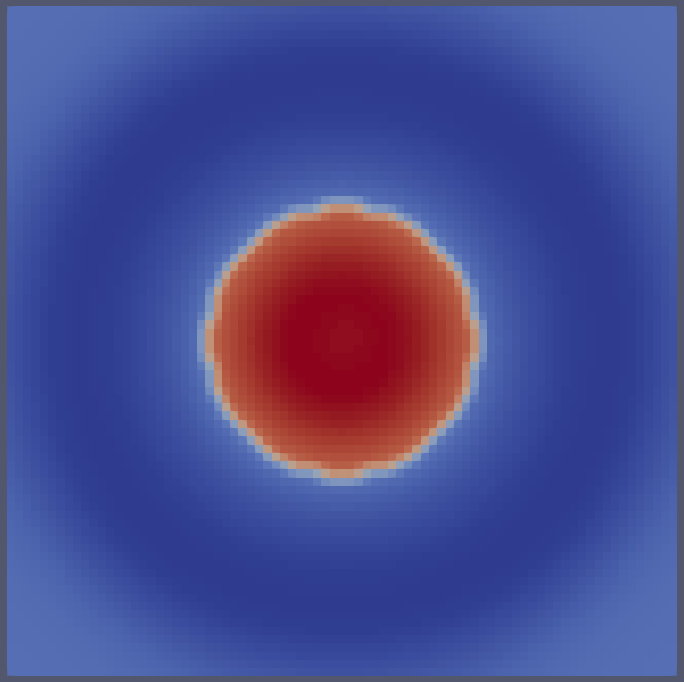
\includegraphics[height=0.48\linewidth]{pictures/SWE_end.png}
\caption{The computed height of the fluid according to our computation of the shallow water equations after 0.2s. The fluid has rushed in from the sides in order to fill the depression at the centre.}
\end{figure}

\newpage


\section{Mesh width and mesh refinement}
\label{refinement}

\vspace{0.2cm}

If you've completed the previous exercice, you may have noticed that the resolution is somewhat low. We're interested in increasing the resolution so we can see more details in the solution. This means we need to consider our cell size, so in a first step we will discuss how the cell size is calculated. For this, we return to the specification file. In particular, we will take another look at the solver definition:\\

\begin{lstlisting}[style = Python]
thesolver = exahype2.solvers.fv.rusanov.GlobalAdaptiveTimeStep(
    "swe",
    patch_size=3,
    unknowns=3, auxiliary_variables=1,
    min_volume_h=0.02, max_volume_h=0.06,
    flux = exahype2.solvers.fv.PDETerms.User_Defined_Implementation,
    ncp = exahype2.solvers.fv.PDETerms.User_Defined_Implementation,
    time_step_relaxation = 0.1
)
\end{lstlisting}

The parameter that interests us here is \textbf{max\_volume\_h}. This determines the maximal allowable size for cells in our volume, in essence guaranteeing $max\_volume\_h > cell\_size$.\\
However since Peano is based upon three-partitioning, it refines the domain into $3^d$ cells, where $d$ is the smallest possible integer that satisfies $max\_volume\_h > domain\_size / 3^d$.\\
For our example above, we have set a domain size of $2.0$ in each direction and $max\_volume\_h = 0.05$. The first three-partition of $2.0$ that is lower than $0.05$ is $\frac{2.0}{3^4}\approx0.0247$ this means that there are a total of $3^4=81$ cells in each dimension. Of these, two are used for the boundary conditions, which means there are a total of 79 cells per dimension inside the domain.\\
In total, that makes $79*79=6241$ cells inside the domain, or (with a parameter \textit{max\_volume\_h=0.02}) $241*241=58081$ cells in two dimensions, an increase of a factor 9. However because the smallest admissible timesteps are proportional to the size of the mesh, the overall computational effort increases by total factor of about 27.

In short, if one wishes to increase or decrease the mesh size, one can just modify the parameter $max\_volume\_h$, but one should be aware that this comes at a significant cost.\\
You may have noticed that there is a second parameter $min\_volume\_h$ however, and this parameter logically determines the minimal mesh size. If this parameter is given a value lower or equal to $max\_volume\_h / 3$ (again, three-partitioning), adaptive refinement is switched on, this means the cell size need not be the same in the entire domain.\\
This adaptive refinement must be defined by adding one additional line to the configuration file however:\\

\begin{lstlisting}[style = Python]
thesolver.set_implementation(
    refinement criterion=ExaHyPE2.solvers.fv.PDETerms.User_Defined_Implementation
)
\end{lstlisting}

This line finally explains the last function in the implementation file, that you may have been wondering about:

\vspace{0.2cm}

\begin{lstlisting}[style = C++]
::exahype2::RefinementCommand examples::exahype2::tutorial::swe::refinementCriterion(
  const double * __restrict__ Q, // Q[3+1]
  const tarch::la::Vector<Dimensions,double>&  volumeX,
  const tarch::la::Vector<Dimensions,double>&  volumeH,
  double                                       t
) {
  return ::exahype2::RefinementCommand result = ::exahype2::RefinementCommand::Keep;
}
\end{lstlisting}

\vspace{0.2cm}

There are three valid return values for this function:

\begin{lstlisting}[style = C++]
::ExaHyPE2::RefinementCommand::Keep
::ExaHyPE2::RefinementCommand::Refine
::ExaHyPE2::RefinementCommand::Erase
\end{lstlisting}

which respectively keep, refine or coarsen the mesh refinement for the current cell.\\
In a next step, we will attempt to use these to conditionally refine our resolution of the shallow water equations.

\begin{enumerate}
    \item Use the function \textbf{refinementCriterion()} to selectively refine only the left half of the domain, then re-compile (by running \textbf{make}) and re-run the simulation. Be aware that this may take a little bit of time. Go get a cup of coffee in the meantime, you deserve it.
\end{enumerate}

\begin{figure}[!h]
\centering
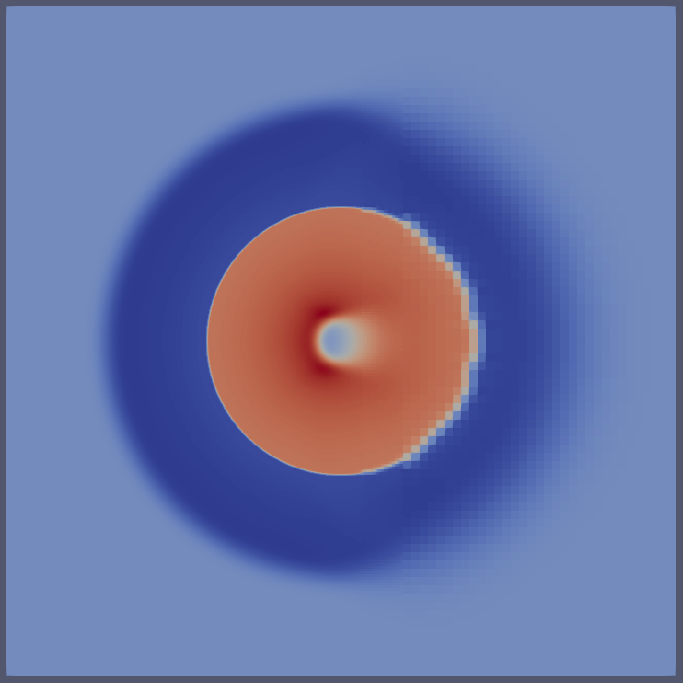
\includegraphics[width=0.45\linewidth]{pictures/SWE_refined.png}
\caption{The shallow water equations with the left half refined.}
\end{figure}

\newpage



\section{The Euler equations}

As a final exercice, we will take a look at a new type of solver for ExaHyPE through the lens of the Euler equations. The Euler equations describe the movement of a fluid if there is neither loss of energy due to frictional forces nor heat conduction in the system. In the finite volume form and given no external forces, the two-dimensional form of the Euler equations appears as follows:

\begin{equation*} \label{Euler_equation}
    \frac{\partial}{\partial t}\left(
    \begin{array}{lr} \rho \\
                      \rho u_1 \\
                      \rho u_2 \\
                      E_t 
                      \end{array} \right) +
    \nabla \begin{pmatrix}
                      \rho u_1          & \rho u_2\\
                      \rho u_1^2 + p    & \rho u_1 u_2 \\
                      \rho u_2 u_1      & \rho u_2^2 + p \\
                      (E_t + p) u_1     & (E_t + p) u_2
    \end{pmatrix}  = \vec{0}
\end{equation*}

where $\rho$ is the density, $u$ is the velocity, $E_t$ is the energy and $p$ is the pressure.\\
The two-dimensional Euler equations have already been implemented in the configuration file Euler2D.py, as well as its corresponding implementation file euler2D.cpp. As before, in order to implement this equation, four things are needed: the initial condition, the boundary conditions, the maximal eigenvalue and the flux. We do not require a non-conservative product.\\

We start with the initial conditions: here we define a starting configuration with a uniform density of \textbf{1.0}, a uniform starting momentum of \textbf{0.0} in both x and y directions and a starting energy that is \textbf{1.0} inside of a circle of radius \textbf{0.2} around the center of the domain and \textbf{1.01} outside of it. Note that we use momentums and not velocities as our variables of choice, this will affect the formulation of some of the equations later.\\

Next we can define the eigenvalues of our system. The eigenvalues of the 2 dimensional Euler equation are:

\begin{equation*}
    \left(
    \begin{array}{lr} \lambda_1 \\
                      \lambda_2 \\
                      \lambda_3
                      \end{array} \right) =
    \left(
    \begin{array}{lr} u - c \\
                      u \\
                      u + c
                      \end{array} \right)
\end{equation*}

where $c$ is the wave propagation speed. For dry air, which can be approximated as an ideal gas, c depends on the pressure as follows:

\begin{equation*}
    \left(
    \begin{array}{lr} \gamma \\
    				  p \\
                      c
                      \end{array} \right) =
    \left(
    \begin{array}{lr}	 1.4 \\ 
					    (\gamma - 1) ( E_t - \frac{1}{2 \rho} (\rho u)^2 ) \\
    					\sqrt[]{\frac{\gamma  p}{\rho}}
                      	\end{array} \right)
\end{equation*}


Finally, we can define our boundary conditions. You can choose any boundary conditions you prefer but we have chosen to use reflecting boundary conditions, this means the values outside of the boundary are the same as the values inside of the boundary.

\newpage

Now that we know what our equations look like, we can take a look at the configuration and implementation. As we've already mentioned, we are using a different solver for this example, this time we have replaced our finite volume solver with an \textbf{Ader-DG} solver. Let's check our configuration file \textbf{Euler2D.py} to see what has changed:\\

\begin{lstlisting}[style = Python]
theSolver=exahype2.solvers.aderdg.rusanov.GlobalAdaptiveTimeStep(
    name="euler+"str(dimensions)+"D",  order=3,
    unknowns=4, auxiliary_variables=0,
    min_cell_h=0.03, max_cell_h=0.1, time_step_relaxation=0.9
)
\end{lstlisting}

All we have had to modify is the solver itself, the definition of project and domain has remained the same, and even our solver looks very similar to before. This was always a key goal of ExaHyPE, we want users to be able to play around with solvers themselves and try out for themselves different ways to solve their equations. The implementation files also have the same structure, this means you can use the same implementation file with different solvers.

And finally, just to make sure we understand what we are doing, we can implement the Euler equations in three dimensions.

\newpage



\section{The three-dimensional Euler equations}
\vspace{0.2cm}
The three-dimensional Euler equation are very similar to the two-dimensional example:

\begin{equation*}
    \frac{\partial}{\partial t}\left(
        \begin{array}{lr}
                    \rho \\
                    \rho u_1 \\
                    \rho u_2 \\
                    \rho u_3 \\
                    E_t 
        \end{array} \right) +
    \nabla
        \begin{pmatrix}
            \rho u_1          & \rho u_2            & \rho u_3\\
            \rho u_1^2 + p    & \rho u_1 u_2        & \rho u_1 u_3 \\
            \rho u_2 u_1      & \rho u_2^2 + p      & \rho u_2 u_3 \\
            \rho u_3 u_1      & \rho u_3 u_2 + p    & \rho u_3^2 + p \\
            (E_t + p) u_1     & (E_t + p) u_2       & (E_t + p) u_3
        \end{pmatrix}  = \vec{0}
\end{equation*}

This has the same eigenvalues as the 2D solution:
\begin{equation*}
    \lambda = \left( \begin{array}{lr}
                     u-c \\
                     u \\
                     u+c \\
        \end{array} \right)
\end{equation*}

And you can use the same approximation for the pressure and wave velocity:
\begin{equation*}
    \left( \begin{array}{lr}
            \gamma \\ 
            p \\ 
            c \end{array} \right) =
    \left( \begin{array}{lr}
                     1.4 \\
                     (\gamma - 1) * ( E_t - \frac{\rho \|u\|}{2} ) \\
                    \sqrt[]{\frac{\gamma  p}{\rho}} \\
        \end{array} \right)
\end{equation*}

\begin{enumerate}
    \item     
        First, create a specification file \textbf{Euler3D.py}. You can start with a copy of \textbf{Euler2D.py}, what will you need to modify?
    \item
        Second, build the project.\\
        Once your project has been built, you will need to implement the functions in the new file \textbf{euler3D.cpp}. You can take inspiration for this from \textbf{euler2d.cpp}.
    \item Once again, be aware that the three-dimensional example may take longer than the two-dimensional example to compute, especially on older hardware.
\end{enumerate}

If at any time you are stuck and incapable of finding an answer, a solution is provided in the directory \textbf{example\_solutions}.

\begin{figure}[!h]
\centering
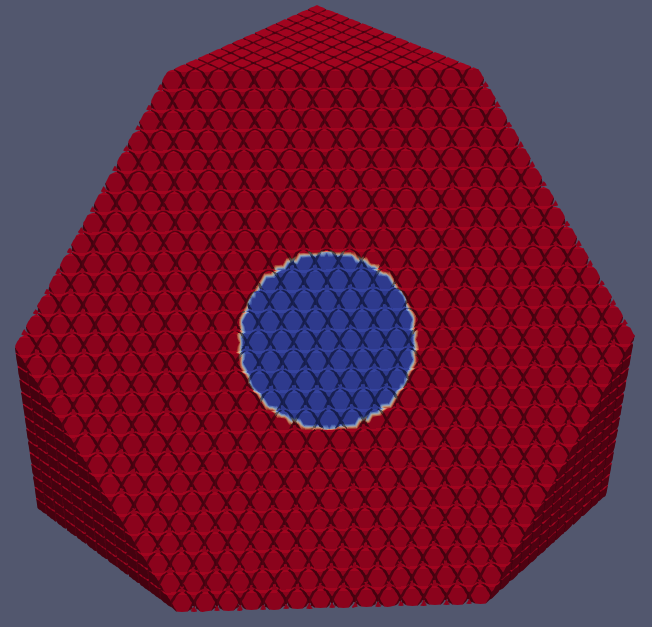
\includegraphics[width=0.40\linewidth]{pictures/Euler_3D_start.png}
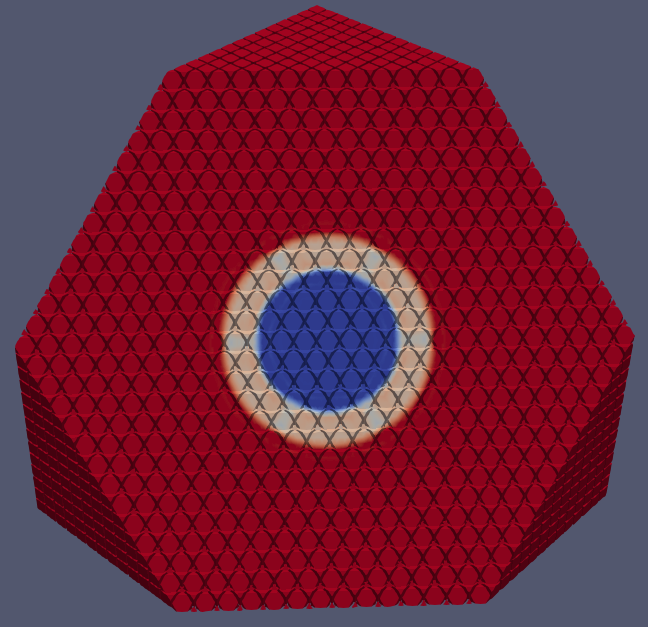
\includegraphics[width=0.40\linewidth]{pictures/Euler_3D_end.png}
\caption{The computed energy of the 3D Euler equations at times t=0.0 and t=1.0}
\end{figure}

\end{document}
